\pdfoutput=1
\pdfmapfile{+cm.map}
\documentclass{llncs}
\usepackage{graphicx,booktabs,amsmath,amssymb,placeins}
\usepackage[hidelinks]{hyperref}
\pdfinfoomitdate=1\pdftrailerid{}
\hypersetup{pdftitle={Solar-Access-Priority Screening: Supplementary Decision Experiment and Revision Options},pdfauthor={},pdfcreator={LaTeX}}
\newcommand{\ind}{\mathbf{1}}
\newcommand{\aidraft}{\footnote{AI-assisted preparation~\cite{openai2026}; scope is stated in the AI Use Disclosure.}}
\setlength{\emergencystretch}{2em}
\renewcommand{\textbullet}{\ensuremath{\bullet}}\renewcommand{\textperiodcentered}{\ensuremath{\cdot}}
\begin{document}
\title{Solar-Access-Priority Screening:\\Supplementary Decision Experiment and Revision Options}
\author{}\institute{}\maketitle\renewcommand{\thefootnote}{\arabic{footnote}}
\begin{abstract}
Solar-access repair should prioritize sunlight improvement before minimizing nominal building intervention. We test whether a ten-candidate shortlist can retain more high-ranked alternatives under that objective than a historical fixed-weight list. A prospectively frozen experiment uses 630 archived two-building height-reduction candidates, three constrained weight spaces, three minimum-area-benefit filters, and independent training, test and replication weights. Two acceptability-based selectors maximize empirical top-ten recovery, with or without protection of observed training winners. None of six contexts satisfies the predeclared conditions for replacing the historical method: recovery gains remain below 0.02, and some lists reduce mean area or duration benefits beyond the declared guard. Nevertheless, useful conditional effects occur. Under a 70\% total sunlight-weight constraint, winner coverage increases from 89.08\% to 100\%, and continuous worst-case normalized regret decreases from 0.019380 to zero. Under ordered weights, the historical list already has zero regret. A stringent area filter leaves only twelve candidates and conceals opportunity loss if evaluated only within that subset. These are new decision analyses of archived performances, not new physical simulations. This supplementary report preserves the prior manuscript and provides evidence-based revision choices; it is not a replacement submission manuscript or a claim of a new general algorithm. AI assistance is disclosed~\cite{openai2026}.
\keywords{Solar access \and Decision support \and Preference sensitivity \and Candidate screening \and Negative results}
\end{abstract}

\section{Research Decision and Scope}
The author has clarified the project objective: improve insufficient sunlight in a dense existing urban block first, prefer smaller interventions second, and leave final design selection to architects.\aidraft{} This is a different decision contract from unrestricted uncertainty over all benefit--cost weights. A method that protects a very low-volume alternative with almost no sunlight benefit can be useful under an open preference model while being poorly aligned with solar-access repair.

The previous experiment used the same 630 archived candidates and found that a greedy regret-oriented Robust10 improved opportunity preservation over the full weight simplex. It also found that the historical top ten already had zero regret over ordered sunlight-priority and local historical spaces, while Robust10 recovered fewer members of preference-specific top tens. Those findings are retained, not reinterpreted as proof of superiority under the author's new priority.

The present question is narrower: can ten review slots preserve more highly ranked sunlight-priority alternatives without losing a best option or sacrificing too much sunlight benefit? The answer must be determined by independent evaluation. The prospective replacement criteria failed in every tested context. Therefore this report documents the new experiment and revision options while preserving the prior formal manuscript. Retention is an archival decision, not an endorsement of submitting that manuscript unchanged under the newly clarified framing.

The outcome is not ``nothing improved.'' Several selectors improve winner coverage in duration-dominant sunlight scenarios, and all new lists improve or match empirical recovery. The important distinction is between a measurable conditional benefit and the stronger, predeclared claim that a new method merits replacing the historical shortlist. Changing the success threshold after seeing those small gains would erase that distinction.

\section{Evidence, Metrics and Established Foundations}
\subsection{Frozen Physical Evidence}
The canonical model contains 45 building groups, of which 36 satisfy the archived research eligibility flags and height condition.\aidraft{} Every unordered pair receives the same fixed-footprint height-reduction rule, giving $\binom{36}{2}=630$ candidates. Selected heights are
\begin{equation}
 h_i^r=\max\{3,h_i-\min(3,0.25h_i)\}.
\end{equation}
Unselected heights and all footprints remain fixed. Eligibility is not permission to demolish, an assessment of ownership or a structural feasibility decision. Footprints are unions of component bounding boxes with known overlap and representation limitations; they are not verified as-built boundaries.

Archived direct-sun duration uses 2,031 receivers on a 3~m grid at 0.1~m height, a near-solstice 21 December 2026 design-day scenario, and sixteen half-hour sample centres between 08:15 and 15:45. Let $D_j^0$ and $D_j(i)$ be baseline and candidate durations. With cell area $a=9$~m$^2$, $P=2031$ and research threshold $\tau=3$~h,
\begin{align}
 A_i&=a\sum_j[\ind\{D_j^0<\tau\}-\ind\{D_j(i)<\tau\}],\\
 H_i&=P^{-1}\sum_j[D_j(i)-D_j^0],\\
 V_i&=\sum_b |F_b|[h_b-h_b(i)],\\
 N_i&=a\sum_j\ind\{D_j^0\geq\tau,\ D_j(i)<\tau\}.
\end{align}
Thus $A$ is net low-sun-area reduction, $H$ mean exposure gain, $V$ nominal additive removal volume, and $N$ newly low-sun area. $V$ is neither a verified whole-scene union-volume change nor a measured construction cost. The exposure threshold is not claimed as a legal compliance test.

The new run verifies exactly $N=0$ for all 630 archived rows. It is omitted from active ranking discrimination but retained as a translation-validity signal. Global normalization bounds remain $A\in[0,396]$~m$^2$, $H\in[0,0.06351551]$~h and $V\in[387.382435,10891.474418]$~m$^3$ (printed rounding; calculations retain the complete archived precision). No bound is refitted after filtering. Define normalized benefits
\begin{equation}
 x_i=(n_{A,i},n_{H,i},1-n_{V,i}),\qquad u_i(w)=w^\top x_i.
\end{equation}
The unchanged historical score is
\begin{equation}
 S_i=.45n_{A,i}+.35n_{H,i}+.15(1-n_{V,i})+.05(1-n_{N,i}).
\end{equation}
Its effective three-criterion centre is $(9/19,7/19,3/19)$, since $S_i=.95u_i(w^0)+.05$. This algebra preserves ordering; it does not validate the weights as architect preferences. $A$ and $H$ are related but distinct: their archived Pearson correlation is 0.640978 and Spearman correlation is 0.768360. One measures threshold crossings, the other duration changes across all receivers.

\subsection{What Is Established Mathematics?}
MCDA provides a mature framework for multiple criteria and incomplete preferences~\cite{GrecoEhrgottFigueira2016}. SMAA-2 examines rank acceptability across preference conditions~\cite{LahdelmaSalminen2001}, with established Monte Carlo implementations~\cite{TervonenLahdelma2007}. We use a restricted fixed-performance version: sampled weight frequencies are properties of a declared integration measure, not probabilities that real architects prefer an option.

Robust ordinal regression uses preference information to restrict compatible additive value functions~\cite{GrecoMousseauSlowinski2008}. No elicited pairwise architect comparisons are available here, so imposing weight inequalities is not fitting an ordinal-regression model. Minimax regret and representative subsets are also established~\cite{BoutilierEtAl2006,NanongkaiEtAl2010}. Their theoretical guarantees cannot be transferred automatically to this finite, normalized absolute-regret implementation.

Building-performance optimization, designer-led massing exploration and urban solar optimization all have substantial precedents~\cite{NguyenReiterRigo2014,WangJanssenJi2024,LiHeZhao2024,LiuEtAl2023}. The solar metrics literature distinguishes exposure, irradiation, daylight and their normalization~\cite{czachura2022metrics,compagnon2004urban}. The possible contribution here is the explicit solar-priority decision formulation, controlled comparison and connection to evidence states in one constrained intervention case. It is not the invention of SMAA, Pareto screening, regret minimization, or architect-in-the-loop design.

\section{Prospectively Frozen Experiment}
\subsection{Three Meanings of Sunlight Priority}
The protocol was committed before any new threshold count, weight draw, ranking or shortlist outcome.\aidraft{} Let $W=\{w\geq0:\sum_jw_j=1\}$. Three primary spaces are
\begin{align}
 W_O&=\{w\in W:w_A\geq w_H\geq w_V\},\\
 W_{70}&=\{w\in W:w_A+w_H\geq.70\},\\
 W_{80}&=\{w\in W:w_A+w_H\geq.80\}.
\end{align}
Ordered weights prioritize the normalized area coefficient over duration and volume. Total-sunlight constraints instead cap the volume coefficient while allowing duration to dominate area. Neither formulation is strict lexicographic optimization of sunlight, and neither guarantees a minimum physical area benefit. The 70\% and 80\% bounds are research scenarios, not industry standards.

Three layered contexts use $W_{70}$ after requiring $A\geq90$, $180$ or $270$~m$^2$. These round multiples of the 9~m$^2$ cell were frozen prospectively. They are minimum-benefit scenarios, not regulations or surveyed expert thresholds. The surviving universes contain 166, 50 and 12 candidates respectively, compared with 630 in each unfiltered context. Raising a floor can remove an otherwise useful duration-beneficial candidate; success within the smaller universe must not conceal that loss.

\subsection{Independent Samples and Equal Budgets}
Each primary space has 20,000 training, 20,000 test and 20,000 replication weights. NumPy PCG64 generates float64 IID Dirichlet$(1,1,1)$ draws. Sorting exchangeable coordinates gives uniform area in the ordered sector. Rejection with $w_V\leq.30$ or $.20$, using batches of 100,000 and retaining accepted draws in order, gives uniform area in each truncated simplex. Seeds are 2026101901--03 for training, 2026101911--13 for test, and 2026101921--23 for replication, in ordered, Solar70, Solar80 order. Layered contexts reuse the exact Solar70 arrays, enabling paired comparisons without pretending they are additional independent preference samples. There are 180,000 unique retained weights.

Every utility ranking uses unrounded values and ascending natural pair identity for exact ties. All six comparators receive ten slots. In the three primary contexts, Historical10, prior Robust10, AV10 and AHV10 are unchanged archived lists. AV10 and AHV10 are historically ranked truncations of their respective Pareto fronts, not optimized ten-member Pareto representatives.

Filtered comparisons explicitly adapt those baselines. Historical10 takes the highest historical-ranked eligible ten. Robust10 retains eligible prior members in insertion order and fills remaining slots by historical rank. AV10 and AHV10 recompute fronts inside the eligible universe, truncate by historical rank, and pad by historical-ranked nonfront members if needed. Original-list threshold violations are separately retained. These are labeled adaptations, not the original lists silently relabeled as feasible. Every filtered universe has at least ten candidates.

\subsection{Two Selection Objectives}
Let $T_{10}(w)$ be the deterministic preference-specific top ten. For a ten-member set $S$, expected recovery is
\begin{equation}
 Q(S)=\mathrm E\left[\frac{|S\cap T_{10}(w)|}{10}\right]
 =\frac1{10}\sum_{i\in S}\Pr\{i\in T_{10}(w)\}.
\end{equation}
Linearity of expectation makes this objective modular. Coverage10 therefore takes the ten largest training top-ten counts. Ties use training winner count, then smaller training mean rank, then natural pair identity. This is exact empirical optimization of the stated objective, not a new general algorithm or proof of optimal population recovery.

ProtectedCoverage10 additionally requires every distinct deterministic training winner to be included. It fills the remaining slots in the same acceptability order. When the required set has at most ten elements this exactly solves the constrained empirical modular problem. If it had more than ten, the frozen rule would declare infeasibility rather than invent a fallback. No test, replication, grid or continuous-audit winner can change selection. In the actual run both methods produce identical memberships in every context: the recovery-optimal lists already contain the observed training winners. Thus there is no observed incremental benefit to the protection constraint here.

Recovery is different from any-top-ten coverage, winner coverage, architectural diversity, or regret. For the eligible universe $D_c$,
\begin{equation}
 R_c(S,w)=\max_{i\in D_c}u_i(w)-\max_{s\in S}u_s(w).
\end{equation}
A list can have zero regret while recovering few other top-ranked candidates. Conversely, maximizing recovery alone does not generally guarantee preservation of every possible winner.

\subsection{Evaluation, Stability and Claim Gates}
Held-out comparisons report deterministic and utility-based winner coverage, mean and worst observed regret, recovery, any-top-ten coverage, raw list and scenario-chosen $A/H/V$ distributions, and archived review coverage. Paired scenario-level differences use sample standard errors and normal 95\% Monte Carlo intervals. These intervals characterize integration precision conditional on fixed inputs and distributions, not cross-site or human-preference uncertainty.

For each selector, ten disjoint 2,000-weight training blocks independently reselect a list. Block-to-full and pairwise Jaccard overlaps describe sensitivity of membership to training samples. This diagnostic never alters the full-training list. A 5,151-point simplex grid, restricted to each space, probes boundaries independently of selection.

A fixed-set continuous audit maximizes, for every eligible candidate $i$,
\begin{equation}
 \max_{w,t}\ t\quad\text{subject to }w\in W_c,\quad
 t\leq w^\top(x_i-x_s)\ \text{for all }s\in S.
\end{equation}
Taking the maximum over $i$ gives continuous worst-case regret for that fixed list and universe. HiGHS uses primal and dual tolerances $10^{-9}$; witnesses and direct regret are checked within $10^{-8}$. There are 10,504 actually executed candidate LPs after deduplicating identical set/space/universe combinations, corresponding to 12,708 labeled witness rows. All solve successfully. This is a fixed-set audit, not a proof of globally optimal shortlist construction.

For layered contexts, the full-universe loss is decomposed rather than hidden:
\begin{align}
 F_c(w)&=\max_{i\in D}u_i(w)-\max_{i\in D_c}u_i(w),\\
 R_{\rm total}(S,w)&=F_c(w)+R_c(S,w).
\end{align}
A zero conditional regret does not imply a zero loss relative to all 630 alternatives.

The protocol permits a supported replacement claim only if ProtectedCoverage10 gains at least 0.02 absolute recovery in both test and replication, with positive paired interval lower bounds; loses no utility winner coverage beyond $10^{-4}$; increases neither mean nor continuous worst regret beyond $10^{-8}$; and retains at least 95\% of both historical-list mean $A$ and mean $H$. The 0.02 and 95\% gates are declared analytical safeguards, not expert-validated standards. They were not relaxed after outcomes. A universal superiority claim would require all feasible contexts to pass.

\section{Results and Failure of the Replacement Hypothesis}
\subsection{Same-Budget Comparisons}
Tables~\ref{tab:comparison1} and \ref{tab:comparison2} retain all methods and contexts.\aidraft{} Coverage and Protected have identical membership and results, so their duplicate rows document the lack of an incremental protection effect rather than two independent successes.
\begin{table}[tbp]\centering\small\caption{Independent test comparison on all 630 candidates. All lists contain exactly ten candidates. The final column is the continuous fixed-set maximum, not the largest sampled test loss.}\label{tab:comparison1}
\begin{tabular}{llrrrr}\toprule
Context & List & Recovery & Winner & Mean $R$ & Cont. max $R$\\\midrule
Ordered & Historical & 0.89495 & 1.0000 & 0.000000 & 0.000000\\
Ordered & Prior robust & 0.44436 & 1.0000 & 0.000000 & 0.000000\\
Ordered & AV & 0.29081 & 1.0000 & 0.000000 & 0.000000\\
Ordered & AHV & 0.74141 & 1.0000 & 0.000000 & 0.000000\\
Ordered & Coverage & 0.89938 & 1.0000 & 0.000000 & 0.000000\\
Ordered & Protected & 0.89938 & 1.0000 & 0.000000 & 0.000000\\
Solar70 & Historical & 0.64965 & 0.8908 & 0.000750 & 0.019380\\
Solar70 & Prior robust & 0.45638 & 1.0000 & 0.000000 & 0.000000\\
Solar70 & AV & 0.21158 & 0.6851 & 0.030440 & 0.232558\\
Solar70 & AHV & 0.65683 & 1.0000 & 0.000000 & 0.000000\\
Solar70 & Coverage & 0.66094 & 1.0000 & 0.000000 & 0.000000\\
Solar70 & Protected & 0.66094 & 1.0000 & 0.000000 & 0.000000\\
Solar80 & Historical & 0.65573 & 0.8444 & 0.001073 & 0.019380\\
Solar80 & Prior robust & 0.45071 & 1.0000 & 0.000000 & 0.000000\\
Solar80 & AV & 0.20581 & 0.6897 & 0.031419 & 0.232558\\
Solar80 & AHV & 0.64956 & 1.0000 & 0.000000 & 0.000000\\
Solar80 & Coverage & 0.66946 & 1.0000 & 0.000000 & 0.000000\\
Solar80 & Protected & 0.66946 & 1.0000 & 0.000000 & 0.000000\\
\bottomrule\end{tabular}\end{table}

\begin{table}[tbp]\centering\small\caption{Layered comparison within each filtered universe. Baselines are explicitly adapted; conditional regrets are not full-universe losses. All lists contain exactly ten candidates. The final column is the continuous fixed-set maximum, not the largest sampled test loss.}\label{tab:comparison2}
\begin{tabular}{llrrrr}\toprule
Context & List & Recovery & Winner & Mean $R$ & Cont. max $R$\\\midrule
A90 & Historical & 0.64965 & 0.8908 & 0.000750 & 0.019380\\
A90 & Prior robust & 0.52989 & 1.0000 & 0.000000 & 0.000000\\
A90 & AV & 0.21158 & 0.6851 & 0.030440 & 0.232558\\
A90 & AHV & 0.65683 & 1.0000 & 0.000000 & 0.000000\\
A90 & Coverage & 0.66094 & 1.0000 & 0.000000 & 0.000000\\
A90 & Protected & 0.66094 & 1.0000 & 0.000000 & 0.000000\\
A180 & Historical & 0.69329 & 0.8908 & 0.000750 & 0.019380\\
A180 & Prior robust & 0.70456 & 1.0000 & 0.000000 & 0.000000\\
A180 & AV & 0.60172 & 0.8908 & 0.000750 & 0.019380\\
A180 & AHV & 0.70680 & 1.0000 & 0.000000 & 0.000000\\
A180 & Coverage & 0.70680 & 1.0000 & 0.000000 & 0.000000\\
A180 & Protected & 0.70680 & 1.0000 & 0.000000 & 0.000000\\
A270 & Historical & 0.99662 & 1.0000 & 0.000000 & 0.000000\\
A270 & Prior robust & 0.99662 & 1.0000 & 0.000000 & 0.000000\\
A270 & AV & 0.90000 & 1.0000 & 0.000000 & 0.000000\\
A270 & AHV & 0.90000 & 1.0000 & 0.000000 & 0.000000\\
A270 & Coverage & 0.99662 & 1.0000 & 0.000000 & 0.000000\\
A270 & Protected & 0.99662 & 1.0000 & 0.000000 & 0.000000\\
\bottomrule\end{tabular}\end{table}


Historical10 remains a strong ordered-priority baseline: test recovery is 0.894950 and every preference retains a winner, with zero continuous regret. The new list raises recovery to 0.899380, only 0.004430 absolute. Prior Robust10 retains the same winner but recovers only 0.444360 of the ordered top ten on average. This is the concrete distinction between preserving one opportunity and offering several high-ranked alternatives.

Under Solar70, Historical10 has test winner coverage 0.89080, mean regret 0.000750 and continuous worst regret 0.019380. ProtectedCoverage10 achieves complete test winner coverage and zero continuous regret, while recovery rises from 0.649650 to 0.660935. Solar80 similarly raises winner coverage from 0.84435 to one and recovery from 0.655725 to 0.669465. Higher total sunlight weight does not make the historical ranking uniformly adequate: Solar80 still permits nearly pure duration preferences. The previous ordered-space zero-regret finding cannot be transferred to this different support.

AHV10 also has zero regret in Solar70 and Solar80. Thus eliminating the historical list's missing winner is not unique to the new selector. Its recovery results remain distinct: 0.656835 under Solar70 and 0.649560 under Solar80. AV10 performs poorly when duration is strongly valued, illustrating the cost of screening on area and volume while omitting the second sunlight measure.

\begin{figure}[tbp]\centering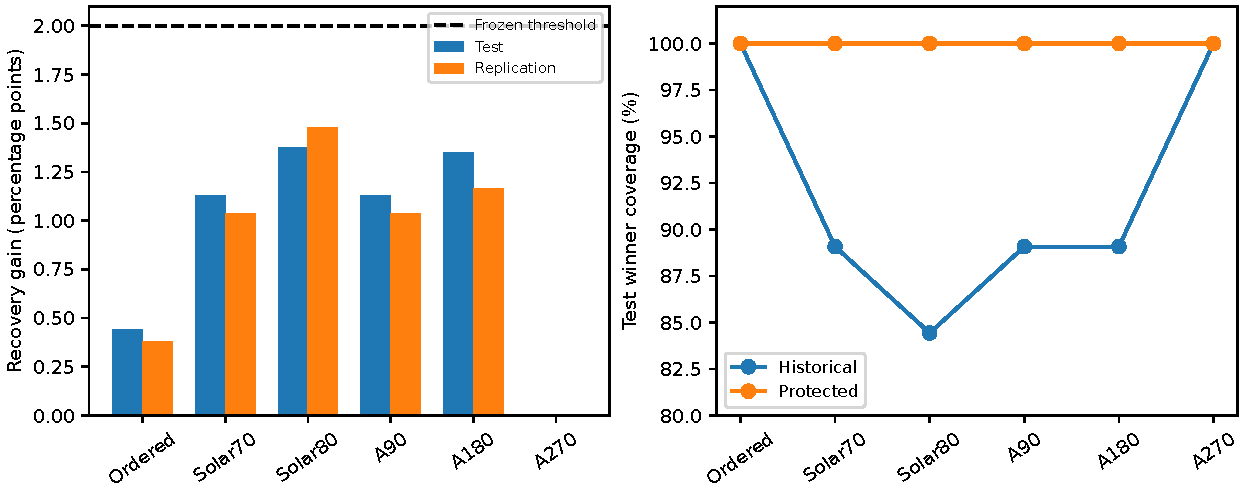
\includegraphics[width=\textwidth]{figures/recovery_and_winners.pdf}
\caption{New computed results from saved CSVs. Left: protected-list recovery gains remain below the frozen two-percentage-point threshold in both independent splits. Right: a real winner-coverage gain occurs in some contexts despite failure of the stronger replacement criterion.}\label{fig:gains}\end{figure}

\subsection{Small Gains, Replication and Solar Trade-offs}
\begin{table}[tbp]\centering\small\caption{Protected minus historical recovery, with paired test Monte Carlo intervals, replication gains and raw list-mean sunlight changes. The frozen replacement threshold is a gain of at least 0.02 in both independent splits.}\label{tab:gates}
\begin{tabular}{lrrrrr}\toprule
Context & Test gain & Test 95\% MC & Repeat gain & $A$ change & $H$ change\\\midrule
Ordered & 0.00443 & [0.00307, 0.00579] & 0.00381 & +3.20\% & -8.23\%\\
Solar70 & 0.01128 & [0.01001, 0.01256] & 0.01038 & -4.36\% & +5.79\%\\
Solar80 & 0.01374 & [0.00972, 0.01776] & 0.01477 & -11.92\% & +18.13\%\\
A90 & 0.01128 & [0.01001, 0.01256] & 0.01038 & -4.36\% & +5.79\%\\
A180 & 0.01350 & [0.01094, 0.01607] & 0.01164 & -7.85\% & +9.68\%\\
A270 & 0.00000 & [0.00000, 0.00000] & 0.00000 & +0.00\% & +0.00\%\\
\bottomrule\end{tabular}\end{table}

No context passes the complete replacement rule. Table~\ref{tab:gates} shows that the positive recovery differences in five contexts are not large enough under the predeclared practical threshold, even when Monte Carlo intervals exclude zero. Statistical integration precision is not practical importance. A270 has no difference at all between the historical and protected sets.

The ordered list replaces C12/C24 with C9/C28. Mean area benefit increases, but mean duration benefit decreases by about 8.2\%, failing the 95\% duration guard. Under Solar80, three substitutions increase duration benefit while reducing mean area benefit by about 11.9\% and increasing nominal mean volume. This is not evidence of improved sunlight repair on every measure, and it is not a cost-saving result. A180 also fails the area guard. Solar70 and A90 pass the raw-mean solar safeguards but remain below the recovery improvement threshold.

\begin{figure}[tbp]\centering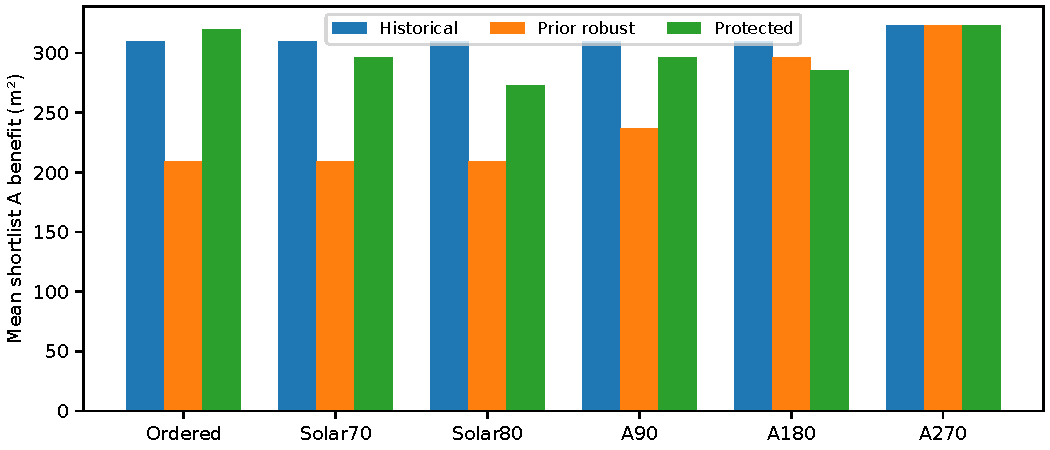
\includegraphics[width=\textwidth]{figures/solar_benefit.pdf}
\caption{Mean raw area benefit of selected lists. Primary contexts use unchanged historical and prior-robust lists. Layered contexts use explicitly adapted versions. A high winner-coverage score does not imply that all ten alternatives have strong area benefits.}\label{fig:solar}\end{figure}

List-average performance is not the outcome of constructing ten interventions, since the architect would choose among alternatives. It is used here as a declared safeguard against offering a generally weak sunlight menu. Scenario-selected best-candidate distributions are also retained, and can differ from list averages. Neither summary replaces individual candidate review or demonstrates human decision quality.

\subsection{The Effect of Hard Minimum Benefits}
A90 removes 464 candidates but leaves the historical and new Solar70 memberships unchanged. Its conditional comparison therefore matches Solar70. A180 leaves fifty candidates and changes several adapted baselines; ProtectedCoverage10 matches AHV10 in this context. These are separate, explicitly filtered decision universes.

A270 leaves only twelve candidates. Historical, prior-robust, Coverage and Protected adaptations become the same ten-member set, with test recovery 0.996625 and zero conditional regret. AV10 and AHV10 remain different and have recovery 0.900000; they must not be described as identical to those four lists. More importantly, the A270 filter itself has mean full-universe opportunity loss about 0.030440 and maximum observed loss about 0.228607 on the Solar70 test weights. A duration-focused preference can lose a valuable candidate before list selection begins. The near-perfect conditional recovery partly reflects a much smaller choice universe, not a universally superior decision method.

No threshold is selected as the ``best'' after seeing these outcomes. An architect might rationally impose a minimum area benefit, but must understand that it expresses a substantive project requirement and may sacrifice duration opportunities. The present experiment exposes that choice rather than authorizing it on the architect's behalf.

\subsection{Membership Stability and Evidence Burden}
\begin{table}[tbp]\centering\small\caption{Protected-list raw means, archived evidence coverage and training-block membership stability. HB denotes rule-level Honeybee review; translation is a separate geometry evidence stage.}\label{tab:evidence}
\begin{tabular}{lrrrrrrr}\toprule
Context & $A$ & $H$ & $V$ & HB & Trans. & $J$ mean & $J$ min\\\midrule
Ordered & 319.5 & 0.03900 & 4378.8 & 9/10 & 3/10 & 1.000 & 1.000\\
Solar70 & 296.1 & 0.04495 & 4427.4 & 9/10 & 3/10 & 0.945 & 0.818\\
Solar80 & 272.7 & 0.05020 & 5350.6 & 7/10 & 2/10 & 0.894 & 0.667\\
A90 & 296.1 & 0.04495 & 4427.4 & 9/10 & 3/10 & 0.945 & 0.818\\
A180 & 285.3 & 0.04660 & 4388.6 & 9/10 & 4/10 & 0.891 & 0.818\\
A270 & 323.1 & 0.03609 & 4288.0 & 8/10 & 3/10 & 1.000 & 1.000\\
\bottomrule\end{tabular}\end{table}

The protected ordered and A270 lists are identical across all training blocks. Solar70 and A90 have mean block-to-full Jaccard 0.945455; Solar80 has 0.893939 and minimum 0.666667; A180 has 0.890909. A small change in average recovery can coexist with changes in marginal membership. These blocks measure numerical sample sensitivity, not repeated architectural projects or users.

\begin{table}[tbp]\centering\small\caption{Illustrative Solar70 protected list, not a newly approved replacement. Membership differs from Historical10 by C24/C35 replacing C9/C27. Position follows the selection record, not a final architectural recommendation.}\label{tab:shortlist}
\begin{tabular}{lrrrrll}\toprule
Pair & Old rank & $A$ & $H$ & $V$ & Rule HB & Trans.\\\midrule
C9/C24 & 1 & 396 & 0.04874 & 5551.3 & Yes & Yes\\
C12/C24 & 7 & 198 & 0.06228 & 4919.3 & Yes & Missing\\
C24/C35 & 11 & 189 & 0.06352 & 6192.0 & Missing & Missing\\
C15/C24 & 4 & 243 & 0.05367 & 4016.5 & Yes & Missing\\
C9/C12 & 3 & 306 & 0.04357 & 4030.5 & Yes & Missing\\
C9/C35 & 5 & 297 & 0.04481 & 5303.3 & Yes & Missing\\
C9/C15 & 2 & 351 & 0.03496 & 3127.8 & Yes & Yes\\
C9/C26 & 9 & 315 & 0.03520 & 3906.1 & Yes & Missing\\
C9/C13 & 6 & 333 & 0.03028 & 2975.2 & Yes & Yes\\
C9/C21 & 8 & 333 & 0.03250 & 4252.0 & Yes & Missing\\
\bottomrule\end{tabular}\end{table}

Solar70 illustrates the useful secondary finding particularly clearly: C24/C35 replaces C9/C27, adding the largest archived duration gain, but has no archived rule-level Honeybee result. Ordered introduces unreviewed C9/C28. Solar80 contains unreviewed C24/C35, C24/C27 and C24/C26. A180 again lacks C24/C35 review. Even the A270 historical adaptation contains unreviewed C9/C28 and C9/C20, because it is no longer the original fully curated historical ten. A filtered or optimized list does not inherit validation merely from its method name.

\section{Simulation and Geometry Remain Separate Evidence}
The new computation consists only of decision analysis on archived $A/H/V/N$.\aidraft{} No new Honeybee/Radiance simulation, physical survey, architect study or construction assessment has been performed. The original 23 curated rule reviews and frozen twenty-candidate same-site coverage sample are preserved without reselection. They total 43 reviewed pairs, not validation of all 630 candidates.

In the archived coverage cohort, area agreement has Spearman correlation 0.997668, with mean absolute difference 0.45~m$^2$ caused by one 9~m$^2$ discrepancy among twenty pairs. This is not sub-grid physical accuracy. Historical score agreement partly shares nominal $V$ and constant $N$ across routes. Honeybee and the screening route also use different effective solar rays; the aggregate agreement does not establish identical physics inputs or generalize to unreviewed pairs.

Historical translated geometries are another stage. Four of five archived translations failed solid containment. Controlled corrections removed observed new obstruction events under the frozen rays and receivers. For C9/C24 the corrected translated area benefit is 351~m$^2$, whereas the rule-screening value is 396~m$^2$. For C9/C15 the corrected translation retains 342~m$^2$, whereas its rule value is 351~m$^2$. Those values concern different geometry and cannot be interchanged in the decision table.

The previously measured implementation speed ratio of about 483 compares two unindexed single-thread Python implementations under matched primitive inputs. It supports the feasibility of rapid finite screening, not superiority over an indexed solver, a new simulation result, or a measured reduction of architects' work time. Ladybug and Radiance provide established simulation context~\cite{roudsari2013ladybug,ward1994radiance}; their names do not certify the input geometry or a proposed intervention.

The evidence sequence remains: rule candidate, selective professional simulation review, translated design and containment checks, then structural, legal and construction feasibility. An architect may use the shortlist to focus attention, but cannot infer completion of later stages from a high score, zero modeled regret or a checked entry in an earlier stage.

\section{Interpretation and Manuscript Revision Options}
\subsection{Answers to the Decision Questions}
The new selectors are more explicit about a particular decision service: retaining multiple high-ranked options across stated sunlight-priority preferences, rather than accepting one unvalidated weight vector.\aidraft{} This gives them interpretability, but does not prove that they are generally better recommendations. In this experiment the gain is too small, or sunlight trade-offs too large, to satisfy the agreed replacement rule.

If Historical10 already includes every winner, as in the ordered space, a new set can add value only through other services such as retaining more near-best options, reducing review burden or improving raw performance. Here the recovery gain is small and mean duration declines beyond the guard. That is not a compelling replacement case. Under Solar70 and Solar80, by contrast, Historical10 does miss some duration-priority winners. Adding those opportunities is a real conditional benefit, but AHV10 and prior Robust10 also retain them, and the new recovery improvement still misses the prospectively declared threshold.

The old broad-space Robust10 lowers mean nominal volume but offers much lower mean area benefit than Historical10 in the primary contexts (208.8 versus 309.6~m$^2$). This does not make its earlier full-simplex regret result false. It shows that unrestricted cost-dominant preferences answer a different question from sunlight-first repair. The correct response is to align the preference model with the project, rather than advertise the largest numerical improvement from an unsuitable weight region.

\subsection{What Should Be Retained or Revised?}
\paragraph{Conservative route.} Preserve the historical shortlist as the default review list, with the newly measured sensitivity and evidence-state annotations. Describe the research as solar-priority interpretable screening and decision support. Its contribution is an explicit constrained decision model, controlled comparison and empirical finding that a plausible new selector fails a stronger replacement test. Do not claim that 45/35/15/5 has thereby become an expert-approved or universally optimal choice.

\paragraph{Conditional route.} If the architect explicitly accepts a total-sunlight space that allows duration-dominant preferences, offer the corresponding alternative list as an optional comparison. Solar70's substitution is easy to explain and merits rule-level review of C24/C35 before design reliance. This is a secondary opportunity-preservation finding, not a reversal of the failed recovery-based replacement test. Choosing this route requires an author decision about the actual decision service, not post hoc threshold relaxation.

\paragraph{Further research.} Elicit real project preferences and rejection constraints; inspect full source literature; perform missing professional simulations only when authorized inputs and environments are available; and study whether architects benefit from these lists. Such work would generate new evidence. It must not be represented as already completed by this preference experiment.

No new formal submission manuscript is substituted in this delivery. The prior English paper and its Chinese versions remain protected in their original location. This supplementary report, complete results and revision options allow the author to choose a justified framing before commissioning a final manuscript revision. The existing paper's broad-space narrative should not be submitted unchanged while presented as proof of sunlight-first superiority.

\subsection{Limitations and Reproducibility}
The analysis uses one simplified site, one fixed rule family, a single day, a coarse receiver grid and fixed archived performances. Weight uniformity, normalization, benefit floors and decision gates are researcher-declared. Correlated sunlight metrics remain compensatory; raw $V$ omits actual cost, relocation, rights and social effects. New weight seeds do not create new site evidence. Repeated evaluation of multiple contexts does not turn conditional Monte Carlo intervals into a familywise scientific discovery test.

All comparisons preserve ten slots, independent selection/evaluation and unfavorable results. The archive contains input hashes, the pre-outcome protocol, software and run logs, retained weights, ranking memberships, candidate acceptabilities, selection traces, continuous-audit witnesses, scenario metrics, stability results and evidence status. The supplementary figures and tables are generated directly from those saved outputs. Physical raw data and the private repository remain restricted; no public replication right is asserted. Author checks of data rights, originality, AI assistance, anonymity and submission declarations remain required.

\section{Conclusion}
None of six prospectively declared contexts supports replacing Historical10 under the complete frozen rule.\aidraft{} Recovery improvements are below 0.02 in both independent splits, and some context-specific lists sacrifice too much mean area or duration benefit. The strongest useful secondary result is more complete winner retention in total-sunlight-weight spaces, including zero continuous conditional regret for the new lists. The strongest warning is that a hard area floor can make within-filter performance look excellent while excluding valuable duration-focused opportunities.

Architects should first clarify whether priority means ordered criteria, a total sunlight emphasis or an explicit minimum area improvement. They can then examine a small annotated set, compare its sensitivities, request missing simulation or geometry evidence, and decide which intervention to develop. The experiment supports that transparent workflow and a cautious default, not an invented algorithm breakthrough or construction-ready recommendation.

\section*{AI Use Disclosure}
An OpenAI assistant~\cite{openai2026} substantially assisted with protocol and code preparation, literature and evidence organization, analysis reporting, equations, drafting, figures, tables, translation preparation and LaTeX quality checks in the abstract and Sections~1--7. Section citations identify assisted text. Charts derive from saved computation; no synthetic observations replace missing physical evidence. The exact underlying model version was not recorded. This statement does not assert completed independent author verification. The author must confirm assistance scope and applicable declarations. An identity-free disclosure is used provisionally because official AI-disclosure and anonymous-acknowledgment instructions require author clarification before submission.
\FloatBarrier\bibliographystyle{splncs04}\bibliography{references}
\end{document}
